In this section, we present most of the machine learning concept utilized in our research.
For more details on the theory in sections \ref{sec:supervised_learning} through \ref{sec:nns}, see \cite{Mehta2019}.

\section{Supervised Learning} \label{sec:supervised_learning}
Supervised learning is a subfield of machine learning that refers to training a model to predict a specific target value based on input data.
In this context, we refer to the input data as "features." The training is supervised when paired with the corresponding target value for prediction.
There are two types of supervised learning, regression and classification. 
In regression, we predict a continuous variable, while in classification predict a binary value, true or false.
The model architecture of the model can be the same regardless of predicting a true/false or continuous value. 
The difference is in the loss function, which is used to evaluate the model's performance during training. The last layer activation function for neural networks is different for regression and classification. 
In-depth explanations of this will come in the following sections.

\section{Loss/Cost} \label{sec:loss_cost}
In machine learning, the loss of a model refers to the discrepancy between the predicted and true values.
It is calculated using a specific function designed to penalize incorrect predictions and measure the model's performance.
The ultimate goal of any machine learning model is to minimize the loss and thereby reduce the difference between predicted and desired outputs.
To achieve this, the model is trained by calculating the gradient of the loss function with respect to different components in the model.
These gradients determine how the model is adjusted to minimize the loss through an iterative process.
As a result, the model is optimized to make better predictions and achieve higher accuracy.\\

The most common loss function for regression is the mean squared error
\begin{equation} \label{eq:mse}
    \mathcal{L}(y, \Tilde{y}) = \frac{1}{N}\sum_{i=1}^N(y-\Tilde{y})^2,
\end{equation}
where $\tilde{y}$ is the prediction, $y$ the true value, and $N$ the number of predictions.

\subsection{Loss Functions}
Loss functions are used to evaluate the performance of the machine learning model during training.
We consider two different loss functions when predicting azimuth and elevation simultaneously with the same model, such as a neural network.
One loss function considers the offset in azimuth and elevation separately, and one considers the total distance.
Let $\Tilde{y}_{Az}$ and $\Tilde{y}_{El}$ denote the prediction for the offset in azimuth and elevation, respectively.
$y_{Az}$ and $y_{El}$ are the true values.
The first loss function is the mean squared error 
\begin{equation}\label{eq:mse1}
    \mathcal{L}_{\text{MSE}} = \frac{1}{2N}\sum_i^N \left( (y_{Az,i}-\Tilde{y}_{Az,i})^2 + (y_{El,i}-\Tilde{y}_{El,i})^2 \right),
\end{equation}
where $N$ is the number of predictions. 
\\
For the second loss function, we use the mean squared distance
\begin{equation}\label{eq:msd}
    \mathcal{L}_{\text{MSD}} = \frac{1}{N}\sum_i^N \left[ (y_{Az,i}-\Tilde{y}_{Az,i})^2 + (y_{El,i}-\Tilde{y}_{El,i})^2 \right],
\end{equation}
It is difficult to predict the effects of these loss functions if any at all, but one difference could be that $\mathcal{L}_{\text{MSE}}$ is more sensitive to outliers,
and $\mathcal{L}_{\text{MSD}}$ reduces the offsets more evenly. \\

For models with a single output azimuth or elevation, we use the regular mean squared error \eqref{eq:mse}

\section{Datasplitting}
Machine learning models can be highly complex and fit all the data points in a dataset.
While this can result in perfect predictions on the training data, it often leads to poor performance on new data, a phenomenon known as overfitting.
To counteract this, the data is typically split into two parts - a training set and a validation set.
The model is trained on the training set, and the error on the validation set is used to evaluate the model's performance. 
By using a separate set of data for validation, we can better estimate the model's performance on new data and avoid overfitting.

When the error on the training data is low, the model has low bias.
However, if the model is too complex, it may also have high variance, meaning that it is overly sensitive to the training data and unable to generalize well to new data.
The key to building a good model is to balance bias and variance and to find the right level of complexity that will allow the model to generalize well.
Proper selection of the train/test split ratio and other techniques, such as regularization, can help achieve this balance and improve the model's performance.

One usually picks the machine learning model with the best performance on the validation set, but this performance is not a reasonable estimate of the expected performance on future predictions.
This is because multiple models are typically trained, and the model with the best performance on the validation set may have obtained its results by chance.
Therefore, a third test set is used to get an unbiased estimate of the model's performance.
The data in the test set is not used when training or validating and is only used to estimate the final model's performance.


\section{Scaling}
In machine learning, some models, such as neural networks, are highly sensitive to the scale of input data.
The inputs to a model often contain different types of data with varying scales.
Neural networks use weights to transform the input data, and each neuron in a fully connected network receives data from every input feature.
If the input features have different scales, training the weights can be slow and unstable.
Scaling the input data to have the same scale improves the speed and performance of the model.
The scaling of the data range does not influence tree-based models, as they operate through binary tests rather than mathematical calculations.
For our research, we scaled the data to have zero mean and a standard deviation of one. This is called standardizing and is achieved by subtracting the mean and dividing by the standard deviation.
Mathematically, the standardization of a feature $x$ is represented as:

\begin{equation}
x_{scaled} = \frac{x - \mu}{\sigma}
\end{equation}

where $\mu$ is the mean of the feature values, and $\sigma$ is the standard deviation of the feature values.
The mean and standard deviation are computed using the following equations:

\begin{align}
\mu &= \frac{1}{n}\sum_{i=1}^{n}x_i\\
\sigma &= \sqrt{\frac{1}{n}\sum_{i=1}^{n}(x_i - \mu)^2},
\end{align}
where $n$ is the number of observations of the feature.
In addition to standardization, other scaling methods, such as min-max and robust scaling, are also used in specific cases.
Overall, scaling is a crucial step in preprocessing data for machine learning, as it can significantly impact the performance of a model.
However, for tree-based methods, scaling has no effect, as predictions are made based on conditions in the data, not mathematical operations.


\section{Decision Trees}
Decision trees are tree-like models that make decisions based on conditions.
As shown in Figure \ref{fig:decitiontree}, each circle represents a node with various types, including decision nodes that split into two other nodes and leaf/terminal nodes that do not.
The root node is the topmost decision node.
Given an observation, a single path to a leaf node represents the prediction made by the decision tree.

Trees are constructed greedily from the top, meaning that each split is made to minimize the loss function at the current step without considering future splits.
More than a single decision tree is required for complex problems.
Various methods exist to improve decision tree models, as Figure \ref{fig:evolution_of_xgb} demonstrates.
The final step in the figure is XGBoost (Extreme Gradient Boost), a highly efficient and high-performing machine learning algorithm.
This section will briefly cover the methods used to optimize decision trees for prediction.

\subsection{Bagging}
Bagging, also known as Bootstrap Aggregation, is a method for training an ensemble of models that contribute to the final prediction.
Each model is trained using bootstrapped data (resampled from the original dataset with replacement), resulting in diverse decision trees.
The final prediction is the average of all ensemble models.

\subsection{Random Forest}
Random forest is based on bagging, where each tree in the ensemble is made using only a randomly chosen subset of features.
This often leads to better generalization and reduced overfitting.

\subsection{Boosting}
In boosting, an ensemble is created, but the trees are not made independently.
They are trained one by one, considering the errors of the previous trees.
A sample weight is assigned to each sample used to train a tree based on the current ensemble's accuracy.
Samples with significant prediction errors are assigned larger weights, and those with accurate predictions are assigned lower weights.
The final prediction is a weighted sum of all ensemble predictions, with weights based on each tree's accuracy.

\subsection{Gradient Boosting}
Like in regular boosting, an ensemble of trees is created iteratively by considering the errors made by previous trees.
The process starts with a constant model that predicts the mean of all samples.
The gradient of the loss function with respect to each sample is calculated, and a tree is made to predict these gradients.
The new prediction is the constant plus a small step in the direction of the predicted gradients.
Repeated iteration with small steps in the gradient direction helps reduce both bias and variance.




\begin{figure}[H]
    \centering
    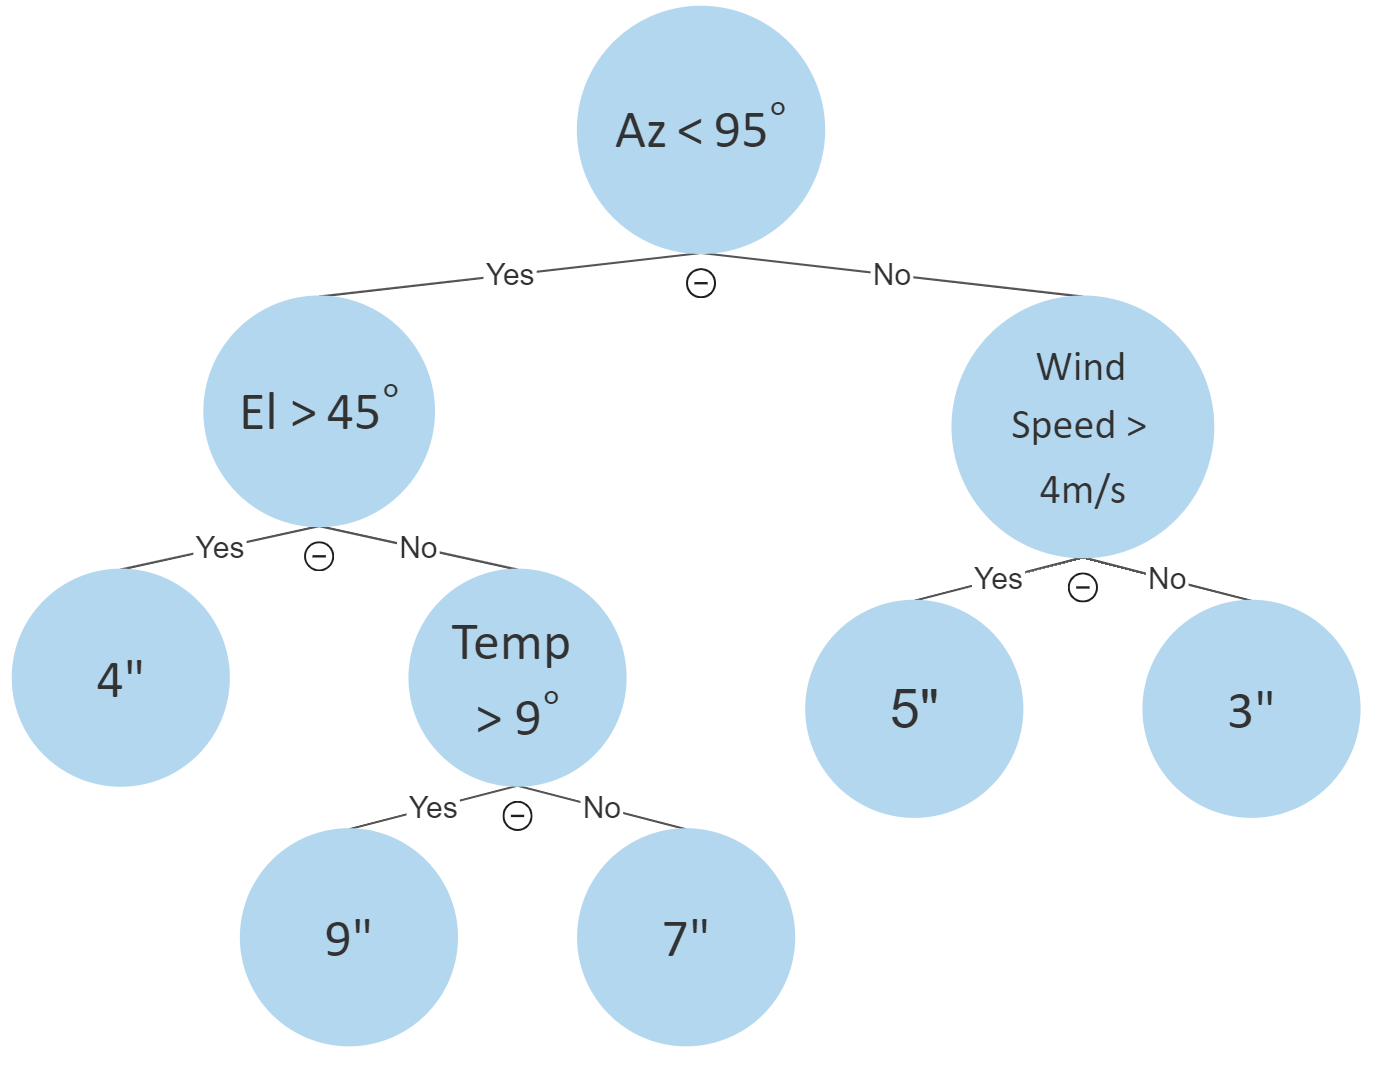
\includegraphics[width=0.8\textwidth]{Other figures/decisiontree_example.PNG}
    \caption[Decision tree]{An example of a decision tree with three decision nodes and five leaf nodes.}
    \label{fig:decitiontree}
\end{figure}

\begin{figure}[H]
    \centering
    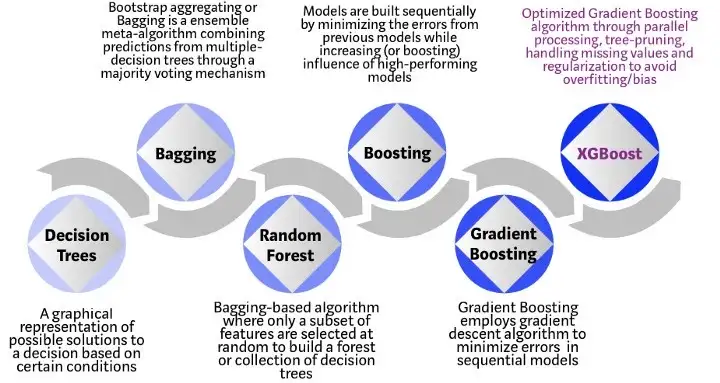
\includegraphics[width=0.98\textwidth]{Other figures/evolution_of_xgb.png}
    \caption[Evolution of XGBoost]{The evolution of XGBoost. Source: \cite{mordevishal}}
    \label{fig:evolution_of_xgb}
\end{figure}

\section{Neural Networks}\label{sec:nns}
A Neural Network (NN) is an Artificial Intelligence (AI) model composed of interconnected neurons inspired by biological neural networks in animal brains.
These networks are arranged in layers, as shown in Figure \ref{fig:nnfig}, and consist of an input layer, one or more hidden layers, and an output layer.
The size of the hidden layer(s) varies depending on the nature of the problem.
A NN processes input to produce an output, ideally close to the true value.

Each connection in an NN has a trainable weight $w_{jk}^l$, representing the weight from the $k^{th}$ neuron in layer $(l-1)$ to the $j^{th}$ neuron in layer $l$.
Each neuron also has its own bias $b_j$, added to its output to prevent the input to its activation function $\sigma$ from being zero.
The activation function $\sigma$ applied to the neuron's output is the final transformation before passing data to the next layer.
This nonlinear function is crucial in allowing NNs to learn nonlinear relationships in data \cite{universalapproximation}.

The following is the mathematical explanation of how a neuron processes the outputs from the previous layer.

\begin{equation} \label{eq:act_neuron}
    a_{j}^l = \sigma\left(\sum_k w_{jk}^l a^{l-1}_k+b_j^l \right) = \sigma(z_j^l)
\end{equation}
The quantity 
\begin{equation}\label{eq:z_neuron}
    z_j^l = \sum_{k} w_{jk}^l a^{l-1}_k+b_j^l
\end{equation}
will be helpful when explaining how to optimize a neural network and can be considered the weighted input for neuron $j$ in layer $l$.


\begin{figure}[H]
    \centering
    % NEURAL NETWORK activation
% https://www.youtube.com/watch?v=aircAruvnKk&list=PLZHQObOWTQDNU6R1_67000Dx_ZCJB-3pi&index=1
\begin{tikzpicture}[x=2.7cm,y=1.6cm]
  \message{^^JNeural network activation}
  \def\NI{5} % number of nodes in input layers
  \def\NO{4} % number of nodes in output layers
  \def\yshift{0.4} % shift last node for dots
  
  % INPUT LAYER
  \foreach \i [evaluate={\c=int(\i==\NI); \y=\NI/2-\i-\c*\yshift; \index=(\i<\NI?int(\i):"n");}]
              in {1,...,\NI}{ % loop over nodes
    \node[node in,outer sep=0.6] (NI-\i) at (0,\y) {$a_{\index}^{(0)}$};
  }
  
 

  % OUTPUT LAYER
  \foreach \i [evaluate={\c=int(\i==\NO); \y=\NO/2-\i-\c*\yshift; \index=(\i<\NO?int(\i):"m");}]
    in {\NO,...,1}{ % loop over nodes
    \ifnum\i=1 % high-lighted node
      \node[node hidden]
        (NO-\i) at (1,\y) {$a_{\index}^{(1)}$};
      \foreach \j [evaluate={\index=(\j<\NI?int(\j):"n");}] in {1,...,\NI}{ % loop over nodes in previous layer
        \draw[connect,white,line width=1.2] (NI-\j) -- (NO-\i);
        \draw[connect] (NI-\j) -- (NO-\i)
          node[pos=0.50] {\contour{white}{$w_{1,\index}$}};
      }
    \else % other light-colored nodes
      \node[node,blue!20!black!80,draw=myblue!20,fill=myblue!5]
        (NO-\i) at (1,\y) {$a_{\index}^{(1)}$};
      \foreach \j in {1,...,\NI}{ % loop over nodes in previous layer
        %\draw[connect,white,line width=1.2] (NI-\j) -- (NO-\i);
        \draw[connect,myblue!20] (NI-\j) -- (NO-\i);
      }
    \fi
  }

  %\node[node] (b1) at (0.8, 1.5) {$b_1$};
  \node[bias] (B) at (0.6,1.8) {$b_j^{(1)}$}; 
  \draw[connect,white,line width=1.2] (B) -- (NO-1);
  \draw[connect] (B) -- (NO-1) node[pos=0.50] {\contour{white}{$b_1$}};

  % INPUT LAYER
  \foreach \i in {2,...,\NO}{ % loop over nodes
    \draw[connect, myblue!20, on layer=back] (B) -- (NO-\i);
    }


  % DOTS
  \path (NI-\NI) --++ (0,1+\yshift) node[midway,scale=1.2] {$\vdots$};
  \path (NO-\NO) --++ (0,1+\yshift) node[midway,scale=1.2] {$\vdots$};
  
  % EQUATIONS
  \def\agr#1{{\color{mydarkgreen}a_{#1}^{(0)}}}
  \node[below=17,right=11,mydarkblue,scale=0.95] at (NO-1)
    {$\begin{aligned} %\underset{\text{bias}}{b_1}
       &= \color{mydarkred}\sigma\left( \color{black}
            w_{1,1}\agr{1} + w_{1,2}\agr{2} + \ldots + w_{1,n}\agr{n} + b_1^{(1)}
          \color{mydarkred}\right)\\
       &= \color{mydarkred}\sigma\left( \color{black}
            \sum_{i=1}^{n} w_{1,i}\agr{i} + b_1^{(1)}
           \color{mydarkred}\right)
     \end{aligned}$};
  \node[right,scale=0.9] at (1.3,-1.3)
    {$\begin{aligned}
      {\color{mydarkblue}
      \begin{pmatrix}
        a_{1}^{(1)} \\[0.3em]
        a_{2}^{(1)} \\
        \vdots \\
        a_{m}^{(1)}
      \end{pmatrix}}
      &=
      \color{mydarkred}\sigma\left[ \color{black}
      \begin{pmatrix}
        w_{1,0} & w_{1,1} & \ldots & w_{1,n} \\
        w_{2,0} & w_{2,1} & \ldots & w_{2,n} \\
        \vdots  & \vdots  & \ddots & \vdots  \\
        w_{m,0} & w_{m,1} & \ldots & w_{m,n}
      \end{pmatrix}
      {\color{mydarkgreen}
      \begin{pmatrix}
        a_{1}^{(0)} \\[0.3em]
        a_{2}^{(0)} \\
        \vdots \\
        a_{n}^{(0)}
      \end{pmatrix}}
      +
      \begin{pmatrix}
        b_{1}^{(1)} \\[0.3em]
        b_{2}^{(1)} \\
        \vdots \\
        b_{m}^{(1)}
      \end{pmatrix}
      \color{mydarkred}\right]\\[0.5em]
      {\color{mydarkblue}a^{(1)}}
      &= \color{mydarkred}\sigma\left( \color{black}
           \mathbf{W}^{(1)} {\color{mydarkgreen}a^{(0)}}+\mathbf{b}^{(1)}
         \color{mydarkred}\right)
         %\color{black},\quad \mathbf{W}^{(0)} \in \mathbb{R}^{m\times n}
    \end{aligned}$};
  
\end{tikzpicture}
    \caption[Neural Network with equations]{This is an illustration of how information is passed through and processed in a neural network.
    Adapted from work by Izaak Neutelings \cite{tikznet}.
    Generated using TikZ \cite{tikz}}
    \label{fig:nnfig}
\end{figure}




\subsection{Backpropagation}
Backpropagation\cite{backprop_original} is a fundamental algorithm in training artificial neural networks.
It calculates the gradient of the loss function with respect to all the weights and biases in the network,
allowing for updating these parameters to reduce the loss.
The algorithm is based on four key equations, which we describe in this section.\\

We define the error in the $j^\text{th}$ neuron in the $l^\text{th}$ layer by
\begin{equation}\label{eq:bp1} 
    \delta_j^l = \frac{\partial C}{\partial z_j^l} = \frac{\partial C}{\partial a_j^l} \sigma '(z_j^l)
\end{equation}

This can also be considered the partial derivative of the cost function with respect to the bias in neuron $j$ in layer $l$, as 

\begin{equation}\label{eq:bp2}
    \delta_j^l = \frac{\partial C}{\partial z_j^l} = \frac{\partial C}{\partial b_j^l} \frac{\partial b_j^l }{\partial z_j^l} = \frac{\partial C}{\partial b_j^l},
\end{equation}
where we have used the relation $\partial b_j^l / \partial z_j^l = 1$ from rearranging equation \eqref{eq:z_neuron}.
The next equation relates the error in a neuron with the errors in the neurons in the subsequent layer.
\begin{equation}\label{eq:bp3}
    \delta_j^l = \frac{\partial C}{\partial z_j^l} = \sum_k \frac{\partial C}{\partial z_k^{l+1}} \frac{\partial z_k^{l+1}}{\partial z_j^l} = \sum_k \delta_k^{l+1} \frac{\partial z_k^{l+1}}{\partial z_j^l} = \left( \sum_k \delta_k^{l+1} w_{kj}^{l+1} \right) \sigma '(z_j^l)
\end{equation}
Note that the indices on the weight $w$ are now swapped.
We may think of this equation as an error propagating backward by multiplying the error in layer $l+1$ with the transpose of the weight connecting layer $l$ with $l+1$
We derive the final equation from the partial derivative of the cost function with respect to the weight $w_{jk}^l$
\begin{equation}\label{eq:bp4}
    \frac{\partial C}{\partial w_{jk}^l} = \frac{\partial C}{\partial z_j^l} \frac{\partial z_j^l}{\partial w_{jk}^l} = \delta_j^l a_k^{l-1}
\end{equation}

Equation \eqref{eq:bp1} lets us calculate the error in the last layer, and using equation \eqref{eq:bp3}, we can propagate this error backward through the network, calculating the error for all the neurons.
We then use equations \eqref{eq:bp2} and \eqref{eq:bp4} to calculate the gradient of the cost function with respect to the weights and biases.


\subsection{Gradient Descent}
Gradient Descent (GD) is an iterative optimization algorithm used in machine learning for minimizing a differentiable function.
The goal of GD is to update the model's trainable parameters in such a way that the loss function is minimized.
In mathematical terms, we aim to find the values of the parameters $\boldsymbol{\theta}$ that minimize the objective function $\mathcal{L}(\mathbf{x}, \boldsymbol{\theta})$, where $\mathbf{x}$ represents the input data.
The loss function is typically defined as the mean squared error \eqref{eq:mse} for regression problems, so
\begin{equation}
    \mathcal{L}(\mathbf{x}, \boldsymbol{\theta}) = \frac{1}{N}\sum_{i=1}^N(y_i-f(\mathbf{x}_i, \boldsymbol{\theta}))^2,
\end{equation}
where $f(\mathbf{x}_i, \boldsymbol{\theta})$ is the output of the model for input data $\mathbf{x}_i$, and $y_i$ is the target value.

To achieve the goal, GD involves calculating the gradient of the loss function with respect to the model's trainable parameters and updating them iteratively by taking a small step in the negative direction of the gradient.
The iterative update rule can be expressed as follows:

\begin{align}
\mathbf{v}_t &= \eta_t \nabla_\theta \mathcal{L}(\mathbf{x}, \boldsymbol{\theta}), \\
\boldsymbol{\theta}_{t+1} &= \boldsymbol{\theta}_t - \mathbf{v}_t,
\end{align}

where $\eta$ denotes the learning rate, and $\nabla_\theta$ denotes the gradient with respect to $\boldsymbol{\theta}$.
The learning rate determines the step size of the update, and it is important to choose a suitable value to ensure convergence of the optimization.

One major limitation of GD is that it can get stuck in local minima, yielding suboptimal results.
The choice of initial parameter values $\boldsymbol{\theta}$ can also impact the final optimized model.
Moreover, computing the gradient using the entire dataset can be computationally expensive for large datasets.
To address these limitations, various modifications of GD have been proposed,
such as stochastic gradient descent (SGD) and mini-batch gradient descent (MBGD),
which compute the gradient using only a subset of the data at each iteration.
These modifications can help to accelerate the convergence and improve the scalability of GD.

\subsection{Stochastic Gradient Descent}
Stochastic Gradient Descent (SGD) is a widely used optimization algorithm in machine learning that addresses some of the limitations of Gradient Descent (GD).
Unlike GD, which computes the gradient using the entire dataset at each iteration, SGD computes the gradient using only a randomly sampled subset, called a mini-batch.
This makes SGD more efficient and less computationally expensive than GD, particularly for large datasets.
Furthermore, by randomly sampling mini-batches, SGD is more likely to escape local minima and converge to the global minimum.
The update rule for SGD can be derived similarly to that for GD, with the only difference being the replacement of the full dataset with a mini-batch.
By iteratively updating the model's parameters using mini-batches, SGD can converge faster and more robustly than GD.

However, SGD also has limitations to consider. If the learning rate is too large, the optimization may overshoot the minimum and fail to converge.
On the other hand, if the learning rate is too small, the optimization may converge very slowly.
In addition, if there are areas in the function space with small gradients, the optimization may stagnate and fail to converge.
To address these limitations, various modifications of SGD have been proposed, such as adaptive learning rate methods like Adagrad and RMSprop,
which adjusts the learning rate dynamically based on the history of the gradients.
These modifications can improve the stability and convergence speed of SGD.


\subsection{Momentum}

In practice, SGD is mostly used with momentum.
Momentum serves as a memory of previous momenta and can improve the convergence speed of SGD, particularly in areas of the function space with low gradients, such as local minima.

The update rule for momentum can be expressed as follows:
\begin{align}
\mathbf{v}_t &= \gamma \mathbf{v}_{t-1} + \eta_t \nabla_\theta \mathcal{L}(\mathbf{x}, \boldsymbol{\theta}) \\
\boldsymbol{\theta}_{t+1} &= \boldsymbol{\theta}_t - \mathbf{v}_t,
\end{align}
where $\gamma$ is the momentum parameter with $0 \leq \gamma \leq 1$.
The momentum term considers the update of the previous step, in addition to the gradients at the current step.
By incorporating previous momenta, momentum can smooth out variations in the optimization trajectory and accelerate convergence towards the minimum.

Momentum is particularly useful when the gradient direction is consistent across many iterations, as it allows the optimization to maintain a higher velocity in the same direction.
In contrast, in areas of high variance or noisy gradients, momentum may cause overshooting and slow down convergence.
To address this, adaptive momentum methods like Adam have been proposed, which adjust the momentum parameter dynamically based on the history of the gradients.
These methods can improve the convergence speed and stability of momentum-based optimization algorithms.


\subsection{Adam}
Adam is an optimization algorithm that combines the benefits of both SGD with momentum and adaptive learning rate methods.
It uses a running average of the first and second moments of the gradient to compute per-parameter adaptive learning rates.
Adam updates the parameters iteratively as follows:

\begin{align}
\mathbf{g}_t &= \nabla_\theta \mathcal{L}(\mathbf{x}, \boldsymbol{\theta}) \\
\mathbf{m}_t &= \beta_1 \mathbf{m}{t-1} + (1-\beta_1) \mathbf{g}_t \\
\mathbf{s}_t &= \beta_2 \mathbf{s}{t-1} + (1-\beta_2) \mathbf{g}_t^2\\
\hat{\mathbf{m}}_t &= \frac{\mathbf{m}_t}{1 - (\beta_1)^t} \\
\hat{\mathbf{s}}_t &= \frac{\mathbf{s}_t}{1 - (\beta_2)^t} \\
\boldsymbol{\theta}_{t+1} &= \boldsymbol{\theta}_t - \eta_t \frac{\hat{\mathbf{m}}_t}{\sqrt{\hat{s}_t} + \epsilon},
\end{align}

where $\mathbf{g}_t$ denotes the gradient at time step $t$, $\mathbf{m}_t$ and $\mathbf{s}_t$ are the first and second moment estimates, respectively.
$\beta_1$ and $\beta_2$ control the decay rate of the first and second moments, respectively.
$\eta_t$ is the learning rate, and $\epsilon$ is a regularization constant to prevent division by zero.

Adam has several advantages over other optimization algorithms, including its ability to adaptively compute per-parameter learning rates and the robustness of its estimates to noise in the gradient.
The adaptive learning rates can help speed up convergence and lead to better performance.
Furthermore, the memory of previous first and second-order gradient estimates enables the algorithm to be more robust to noise and outliers in the data.
As a result, Adam is widely used and has become the de facto standard optimization algorithm in deep learning.


\subsection{Activation Functions}
Activation functions play a crucial role in training a neural network by allowing it to learn non-linear relationships between inputs and outputs.
Different activation functions have varying properties; we will discuss some of the most common ones in this section.
Properties like non-linearity, differentiability, monotonicity, smoothness, and zero-centering are important for activation functions.
Non-linearity enables the model to capture complex relationships, differentiability is necessary for calculating the derivative of the loss function with respect to the trainable weights, monotonicity helps ensure stability in activation outputs, smoothness stabilizes gradients during training, and zero-centering balances the activation distribution within the model.

\begin{itemize}
    \item Non-linearity enables the model to capture complex relationships
    \item Differentiability is necessary for calculating the derivative of the loss function with respect to the trainable weights
    \item Monotonicity helps ensure stability in activation outputs, smoothness stabilizes gradients during training
    \item Smoothness: A smooth activation function helps stabilize the gradients and training.
    \item Zero-centering balances the activation distribution within the model.
\end{itemize}

\subsubsection{Tanh}
Tanh, the hyperbolic tangent function is given by
\begin{equation}\label{eq:tanh}
    Tanh(x) = \frac{e^x+e^{-x}}{e^x-e^{-x}}
\end{equation}

\subsubsection{ReLU}
The Rectified Linear Unit (ReLU) activation function pushes all negative values to zero while leaving positive values unchanged,
which introduces non-linearity while solving the vanishing gradients problem by having a gradient of either 0 or 1 for negative and positive values, respectively.
\begin{equation}\label{eq:relu}
    ReLU(x) = \begin{cases} x & \mbox{if } x > 0 \\ \mbox{0,} & \mbox{otherwise} \end{cases}
\end{equation}

\subsubsection{GeLU}
The Gaussian Error Linear Unit (GeLU) is a smooth approximation of the ReLU function, given by
\begin{equation}
    GeLU(x) = x \Phi (x),
\end{equation}
where $\Phi(x)$ is the standard Gaussian cumulative distribution function.

GeLU can be approximated with
\begin{equation}
    GeLU(x) \approx 0.5x \left( 1+\tanh\left[\sqrt{2/\pi}(x+0.044715x^3)\right] \right),
\end{equation}
which is faster to compute than the original definition but can result in worse performance.
For computational efficiency, we used this approximation.


\section{Model Explainability}\label{sec:model_explainability}
In the context of machine learning, SHAP \cite{SHAP} and SAGE \cite{SAGE} apply the same idea to determine the contribution of each feature to a prediction.
SHAP provides a local explanation by computing the contribution of each feature to the prediction of a single data point.
On the other hand, SAGE provides a global explanation by computing each feature's contribution to the model's overall prediction performance.
These methods allow us to understand the relationship between the features and the prediction, which is particularly useful when the model is too complex to interpret.
Additionally, they provide a way to validate the model's fairness and bias.
By understanding which features contribute the most to a prediction, one can determine if the model is fair or biased and if the prediction is trustworthy.\\

Both SHAP and SAGE methods are based on Shapley values \cite{shapleyvalue1953}, a concept in game theory introduced by Lloyd Shapley in 1951.
Shapley values determine each player's contribution to a group's surplus or overall value.
The explanation below of Shapley values, SHAP, and SAGE is inspired by a blog post by Ian Covert \cite{covertshapsage}, the author of \cite{SAGE}.\\

The Shapley value for a player $i$ in a cooperative game with $d$ players is
\begin{equation}
    \phi_i(w) = \frac{1}{d} \sum_{S \subseteq D \backslash \{ i \} } \binom{d-1}{|S|}^{-1} \left[ w(S\cup \{ i \} ) - w(S) \right]
\end{equation}

where $D$ is the set of all players, $S$ is a coalition of players, $w(S)$ is the value of the coalition $S$, and $|S|$ is the number of players in the coalition.
This formula satisfies four important conditions:
\begin{itemize}
    \item Efficiency: The sum of all Shapley values is equal to the group's total value.
    \item Symmetry: If two players $i$ and $j$ have the same impact on all coalitions with $w(S \cup \{i\}) = w(S \cup \{j\})$ for all $S$, they should have the same Shapley value $\phi_i(w) = \phi_j(w)$.
    \item Dummy: A player $i$ that makes no contribution to the group with $w(S \cup \{i\}) = w(S)$, should receive a value of zero, or $\phi_i(w)=0$.
    \item Linearity: A player's value is proportional to their contribution to the group.
If player $i$ contributes twice as much as player $j$ to the group's overall worth, then player $i$ should have twice the Shapley value.
\end{itemize}

\subsection{SHAP}
Shapley values explain how each feature $(x^1, \dots, x^d)$ in a model $f$ contributes to the deviation from the mean prediction $\mathbb{E}[f(x)]$ of the dataset for a single prediction.
It assigns a value $\phi_1, \dots, \phi_d$ to each feature that quantifies the feature's influence on the prediction $f(x)$.
SHAP (Shapley Additive Explanations) computes approximate Shapley values for machine learning models.\\

We define a cooperative game $v_{f,x}$ to represent a prediction given the features $x^S$, as
\begin{equation}
    v_{f,x}(S) = \mathbb{E} \left[ f(X) | X^S = x^S \right],
\end{equation}

where $x^S$ are known, and the remaining features are treated as random variable $X^{\Bar{S}}$ (where $\Bar{S} = D \backslash S$).
This is the mean prediction $f(X)$ when the unknown values follow the conditional distribution $X^{\Bar{S}} | X^S = x^S$.\\

Using a subset of features from the prediction while sampling the rest from the dataset reduces the chance of improbable samples.
Given this convention for making predictions, we can apply the Shapley value to define each feature's contribution to the prediction $f(X)$ using Shapley values $\phi_i(v_{f,x})$.
A Shapley value of $\phi_i(v_{f,x}) > 0$ indicates that feature $i$ contributes to an increase in prediction $f(X)$.
A negative Shapley value $\phi_i(v_{f,x}) < 0$ indicates the opposite, that the feature contributes to a decrease in $f(X)$.
Uninformative features will have small values $\phi_i(v_{f,x}) \approx 0$.

\subsection{SAGE}
SAGE (Shapley Additive Global Importance) explains how every feature contributes to the model's overall performance, and it relates to SHAP in a simple way.
For a given feature, the global feature importance is the average SHAP value (for that feature) across all samples in the dataset.
This is, however, different from how it is calculated in practice.
A paper by Ian Covert et al.
\cite{sagepaper} on global feature importance proposes an algorithm that aims directly at a global feature explanation, unlike the SHAP values, which makes
it faster.
This is the algorithm used for approximating the SAGE values for the features in the thesis.

\section{Mutual Information}
Mutual information is a fundamental measure of the statistical dependence between two random variables,
providing a way to quantify the amount of information one variable conveys about the other \cite{Shannon1948}.
For a pair of discrete random variables $X$ and $Y$, we have 
\begin{equation}\label{eq:mutual_info}
    I(X;Y) = \sum_{y} \sum_{x} p(x,y) \log \left( \frac{p(x,y)}{p(x)p(y)} \right),
\end{equation}
where $p(x,y)$, $p(x)$, and $p(y)$ are the joint and marginal probabilities, respectively.
The mutual information captures linear and nonlinear relationships between variables, unlike Pearson's correlation coefficient, which can only detect linear relationships.
However, mutual information has limitations in that it relies on binning the data, which can introduce bias and limit the resolution of the information.
   
Furthermore, estimating mutual information for high-dimensional data sets can be computationally expensive.
Despite these limitations, mutual information remains a popular tool in feature selection, data visualization, and machine learning.